% STATUS: WRITTEN, 15 November 2026, against replication factor 3 and strong
% reads throughout. Every number is transcribed from results/recorded/*.csv or
% from the run directories under results/runs/, and every row in those files
% names the run it came from. Objective costs are computed from the recorded
% latency, movement and imbalance with Eq. (1), never by hand from a figure.

\section{Evaluation}

The evaluation answers five questions, in order. Does it matter on real
hardware where a shard's leaseholder sits? Is the gain from moving data a
gain from \emph{choosing} where to move it? How does the room available to a
better policy change as the workload moves faster? Does the learned policy use
that room in simulation? And does what it learned survive the move to a real
cluster?

% ---------------------------------------------------------------------
\subsection{Setup}

The simulated cluster has six regions, one node per region, replication
factor three, and a keyspace of 256 cells from which shards are built. An
episode is 200 decision windows. At each window the policy sees the
per-region read and write counts from the window just finished and issues one
action; the environment then charges it for the latency its placement
produced and for the data any move carried. Reads are strong: they are served
by the leaseholder, which is how the cluster serves a read that is not marked
as stale, so the simulator and the cluster price a read the same way.

Every policy runs through the same episode loop. The policies are static hash partitioning, random relocation, the
reactive heuristic that follows the traffic, a co-location planner modeled on
Lion~\cite{lion2024}, and the learned policy. The Lion-style planner re-plans
every ten windows: it groups shards that are accessed together, places each
group on one region by a cost model that prefers moving a lease over copying
data, and then rebalances load. Beside them sits a per-window bound: the
lowest latency reachable by relocating every lease for free, each window,
\emph{at the shard boundaries the episode started with}. It is not a global
optimum. A policy that moves replicas or splits shards can score below it.

The agent minimises a single cost, which is the quantity it is judged on
throughout:
%
\begin{equation}
c = \frac{\ell}{100} \;+\; w \cdot \frac{g}{2000} \;+\; 0.10 \cdot b
\label{eq:objective}
\end{equation}
%
where $\ell$ is mean transaction latency in milliseconds, $g$ is gigabytes
moved over the episode, $b$ is load imbalance, and $w$ is the migration
weight, 0.30 unless stated. Latency is what we want low, moving data is
charged for, and concentrating the workload on one node is charged for
separately, so that a policy cannot win on latency by overloading a single
region. Migration is expressed as a fraction of the dataset, so the 60\,GB
simulator and the 1\,GB cluster score the same physical move identically.

The agent is a Deep Q-Network with invalid actions masked both at selection
and in the bootstrap target, and three-step returns, so that a move is
credited with the latency it saves in the windows after it. Masking removes
the inapplicable actions that dominated an earlier unmasked agent; across the
runs reported here the inapplicable share is 0.0\%. Each training run takes
$10^6$ steps at volatility 4.

Two seed blocks appear and are never mixed in one table. The volatility sweep
uses seeds 0 to 7. Agent evaluations use held-out seeds 2000 to 2007, which
the training configuration refuses to overlap with its training seeds.

The cluster has six CockroachDB nodes in containers with inter-region
round-trip times injected by \texttt{netem}, on a four-core GitHub Actions
runner, replication factor three. A harness executes each action as a
synchronous relocation statement, reads the resulting placement back from the
database, and only then times $N=200$ transactions issued from per-region
connections. $N$ was chosen by measuring the standard error of the mean
latency, which is about 1 to 2\,ms per episode at that size. Before any
measurement the harness waits until every range has three voters and then
freezes the database's own rebalancer, so the placement under test is the one
the policy chose.

% ---------------------------------------------------------------------
\subsection{Q1: placement changes latency on real hardware}

The gate runs the same transactions twice on the cluster: once with the
leaseholders for the keys involved gathered in the region issuing them, and
once with those leaseholders spread across regions
(Table~\ref{tab:cluster}, Fig.~\ref{fig:cluster}).

\begin{table}[t]
\caption{Cluster gate, replication factor 3, $N=200$ transactions per arm.
Source: \texttt{results/recorded/cluster.csv}.}
\label{tab:cluster}
\centering
\begin{tabular}{lrr}
\toprule
Leaseholders & p50 (ms) & p95 (ms) \\
\midrule
co-located &  293.6 &  441.7 \\
spread     & 1059.0 & 1779.5 \\
\bottomrule
\end{tabular}
\end{table}

\begin{figure}[t]
\centering
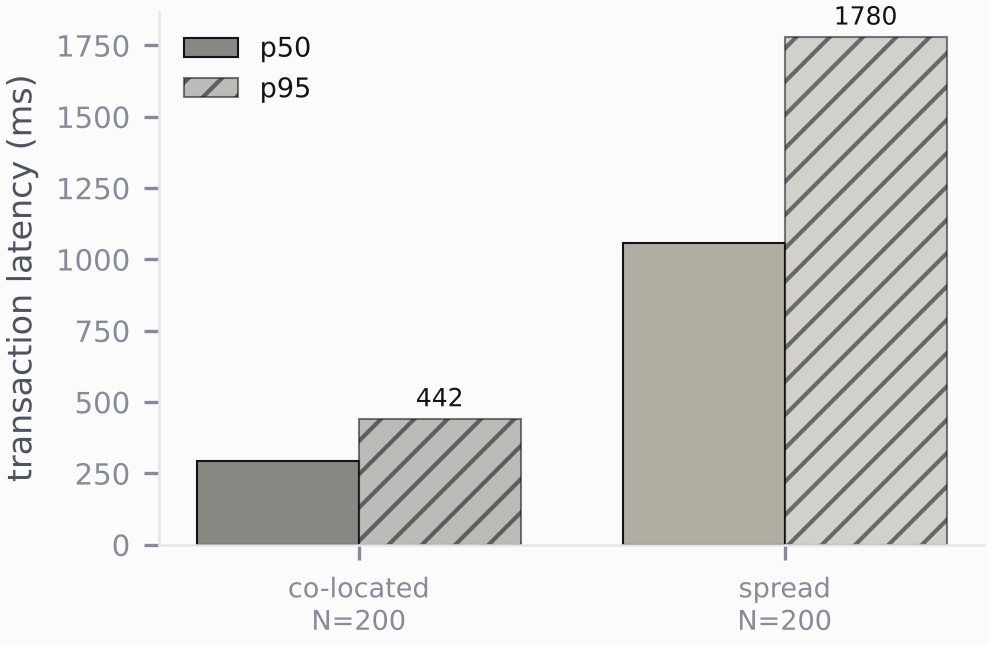
\includegraphics[width=\columnwidth]{cluster.png}
\caption{Co-located against spread leaseholders on the real cluster,
replication factor 3. The difference is far larger than the measurement
noise, which is all this experiment is asked to establish.}
\label{fig:cluster}
\end{figure}

The p95 gap is 1337.8\,ms, with a bootstrap 95\% interval of
[1168.5, 1407.8]\,ms. Placement is worth a great deal on real hardware, which
is the assumption the rest of the work rests on.

Two qualifications belong with that number. First, ``co-located'' means the
leases, not the data. With one node per region the three voters sit in three
regions, so every write still pays a cross-region quorum, which is why the
co-located p50 is 293.6\,ms rather than single digits. What the gate isolates
is the leaseholder effect, which is exactly what the \textsc{move\_lease}
action controls. Second, the co-located arm places every lease on one node,
so it is the arm most exposed to that node saturating. It did not: the
leaseholder node averaged 15.7\% of one core, and the arm's median latency
did not drift across the run. Earlier pilots that suggested saturation had
run on a cluster that had not finished replicating, and are not reported.

% ---------------------------------------------------------------------
\subsection{Q2: the gain comes from choosing, not from moving}

\begin{table}[t]
\caption{Volatility sweep. Mean latency (ms) and data moved per episode
(GB), eight seeds per value, seed block 0 to 7. Source:
\texttt{results/recorded/sweep.csv}.}
\label{tab:sweep}
\centering
\small
\begin{tabular}{lrrrrrr}
\toprule
Vol. & Static & Random & Follow & Lion & Bound & Follow GB \\
\midrule
0.5 & 196.8 & 196.4 & 117.0 & 183.0 & 118.7 & 322.5 \\
1.0 & 196.3 & 201.6 & 119.8 & 181.7 & 118.0 & 632.6 \\
2.0 & 195.5 & 201.6 & 137.4 & 173.3 & 111.5 & 900.2 \\
4.0 & 196.1 & 203.0 & 160.4 & 177.8 & 102.8 & 873.7 \\
\bottomrule
\end{tabular}
\end{table}

The random baseline separates two explanations that are easy to confuse. It
relocates data without looking at the traffic. Across the sweep in
Table~\ref{tab:sweep} it moves 162.7\,GB per episode and ends between 196.4
and 203.0\,ms, no better than doing nothing and at higher volatility slightly
worse. The heuristic, at volatility 1, reaches 119.8\,ms, 39.0\% faster than
static hashing. Movement by itself buys nothing; everything is in the choice
of destination. That is why the problem is a decision problem, and why a
learned policy is a sensible thing to attempt.

% ---------------------------------------------------------------------
\subsection{Q3: the room for a better policy grows with volatility}

Volatility controls how fast the geographic centre of the workload drifts
between windows. Table~\ref{tab:sweep} and Fig.~\ref{fig:sweep} sweep it over
a factor of eight.

Static hashing is flat, 195.5 to 196.8\,ms. It never tracked the workload, so
it does not degrade as the workload moves faster. The bound improves, from
118.7 to 102.8\,ms, because a more volatile workload is a more sharply
concentrated one, and a concentrated workload is easier to serve if the data
is in the right place. Faster drift makes the problem harder for a policy and
easier for an oracle.

The heuristic goes the other way: 117.0\,ms rising to 160.4\,ms, whilst the
data it moves rises from 322.5\,GB to about 900\,GB. Its advantage over static hashing falls from
40.6\% to 18.2\%. A rule that reacts to the window just finished is chasing a
target that has already moved, and under fast drift much of what each move
buys has expired by the time it lands.

\begin{figure*}[t]
\centering
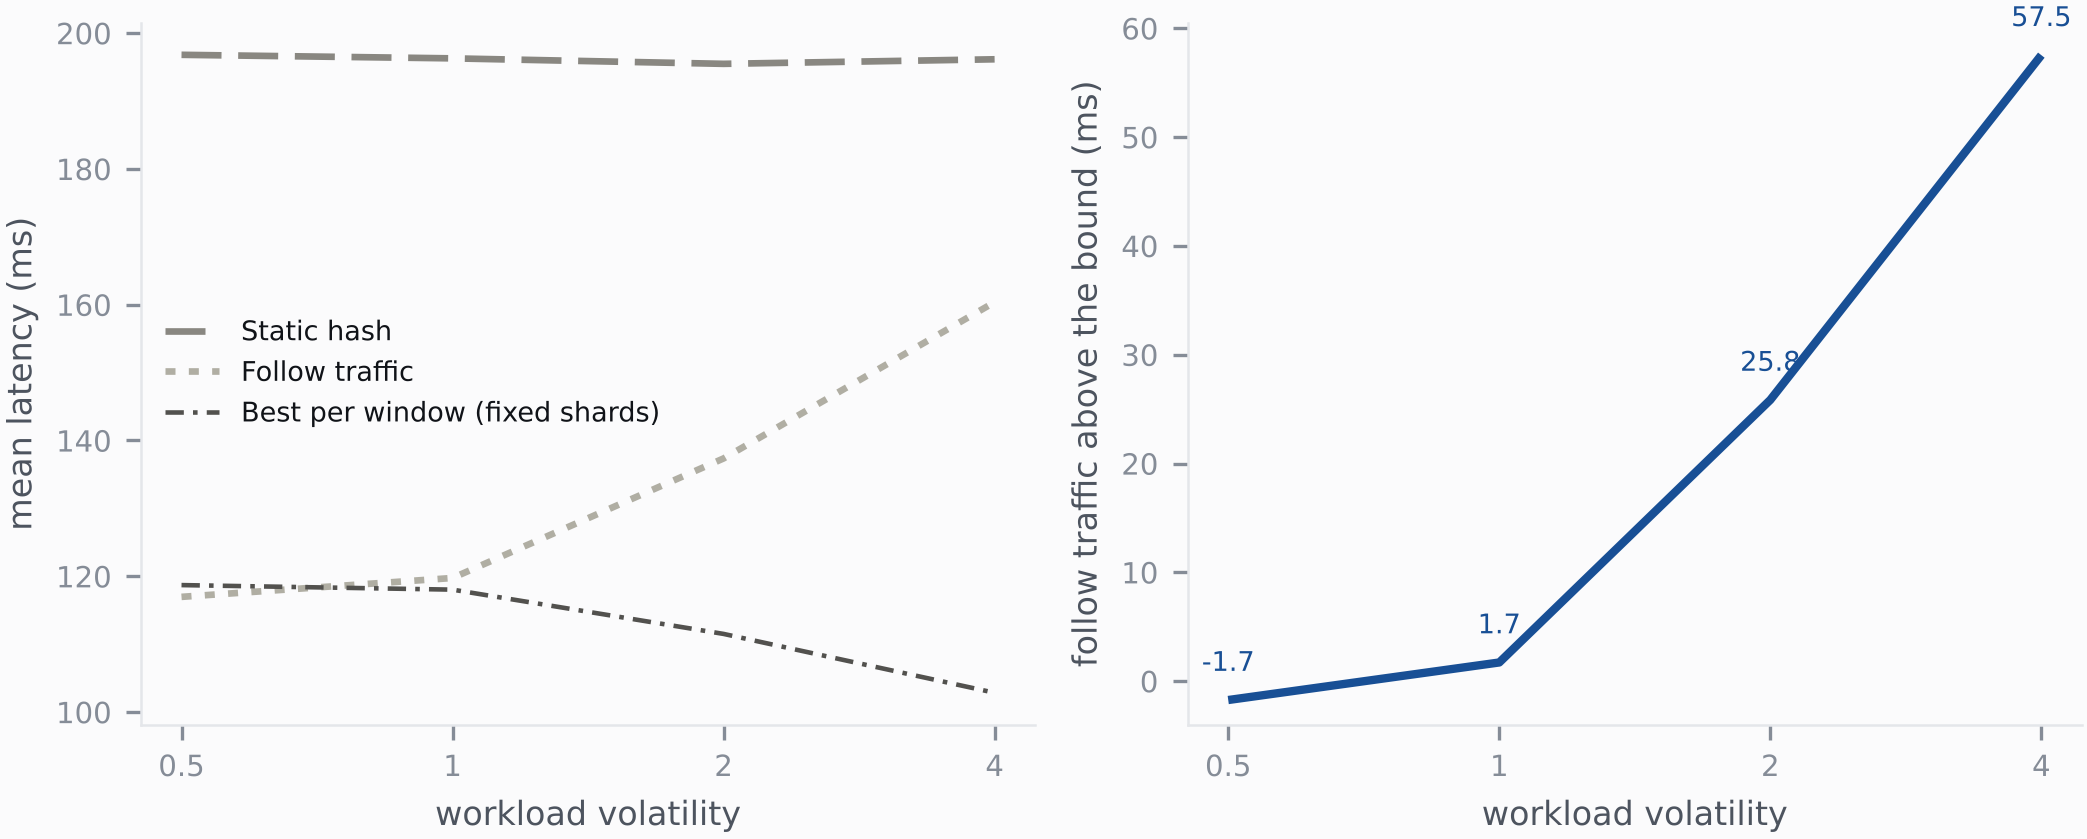
\includegraphics[width=\textwidth]{sweep.png}
\caption{Left: latency against volatility for static hashing, the reactive
heuristic and the per-window bound. Right: the heuristic's distance above the
bound, the room available to a better policy. Seed block 0 to 7.}
\label{fig:sweep}
\end{figure*}


The gap between the heuristic and the bound is $-1.7$\,ms at volatility 0.5,
1.7\,ms at volatility 1, 25.9\,ms at 2 and 57.5\,ms at 4, where it is 36\% of
the heuristic's own latency. At slow drift the heuristic is slightly
\emph{below} the bound, because it moves replicas as well as leases and the
bound moves leases only. Under slow drift, then, a reactive rule is already as
good as the reference, and there is nothing worth learning. Under fast drift
there is a great deal. The case for a learned policy is conditional on
volatility, and the condition is measured rather than assumed. The
Lion-style planner, which re-plans on a fixed period and moves little data
(15 to 24\,GB), sits between static hashing and the heuristic at every
setting.

% ---------------------------------------------------------------------
\subsection{Q4: in simulation the agent trades latency for movement}

Table~\ref{tab:agent} reports four agents trained at volatility 4 from
different learner seeds, evaluated on held-out seeds 2000 to 2007 against
the baselines on the same seeds.

\begin{table}[t]
\caption{Held-out seeds 2000 to 2007, volatility 4, $w=0.30$. Agent rows are
four learner seeds. Source: \texttt{results/recorded/heldout-rf3.csv}.}
\label{tab:agent}
\centering
\begin{tabular}{lrr}
\toprule
Policy & ms & GB moved \\
\midrule
Agent, learner seed 1 & 163.2 & 117.8 \\
Agent, learner seed 2 & 170.7 & 278.1 \\
Agent, learner seed 3 & 162.7 & 121.7 \\
Agent, learner seed 4 & 166.9 & 216.7 \\
\addlinespace
Static hash   & 192.1 &   0.0 \\
Random        & 195.5 & 134.6 \\
Follow traffic& 148.8 & 867.7 \\
Lion-style    & 180.0 &  28.8 \\
Bound         &  91.0 &   0.0 \\
\bottomrule
\end{tabular}
\end{table}

On every learner seed the agent is faster than static hashing, by 13.7\% on
average (165.9 against 192.1\,ms), and faster than the Lion-style planner by
14.1\,ms. It is 17.1\,ms slower than the heuristic and moves 21\% of the
heuristic's data (183.6 against 867.7\,GB on average). It buys its latency
mostly with lease moves, which carry no data: on the cluster episode in Q5,
131 of its 200 actions moved a lease, 55 moved a replica and 14 split a
shard.

Under the objective the comparison with the heuristic is close and goes
against the agent. With the latency and migration terms alone, at $w=0.30$,
the four agents score 1.646 to 1.749 against the heuristic's 1.618; the
imbalance term was not recorded for the agent runs and is omitted from both
sides here. The agent does not beat the heuristic on the objective it was
trained on.

How this verdict depends on the price of movement is the subject of
Table~\ref{tab:weight}. The policies' trajectories are fixed; only the weight
used to score them changes. In simulation, the agent's cost falls below the
heuristic's once $w$ exceeds 0.50, and stays below the Lion-style planner's
until $w$ reaches 1.82. Over that whole band the learned policy is the
cheapest of the four. This is a rescoring, not a retraining: an agent trained
at a higher weight would behave differently, and that experiment has not been
run.

\begin{table}[t]
\caption{Objective cost as the migration weight $w$ varies, with each
policy's behavior fixed. Simulator: held-out seeds, mean of the four agents,
imbalance omitted. Cluster: one episode per policy, full
Eq.~\eqref{eq:objective}. Lowest in each row in bold.}
\label{tab:weight}
\centering
\small
\begin{tabular}{llrrrr}
\toprule
 & $w$ & Agent & Follow & Lion & Static \\
\midrule
Simulator & 0.0 & 1.659 & \textbf{1.488} & 1.800 & 1.921 \\
          & 0.3 & 1.686 & \textbf{1.618} & 1.804 & 1.921 \\
          & 0.6 & \textbf{1.714} & 1.748 & 1.808 & 1.921 \\
          & 1.0 & \textbf{1.751} & 1.922 & 1.814 & 1.921 \\
\addlinespace
Cluster   & 0.0 & 2.008 & \textbf{1.775} & 2.036 & 2.103 \\
          & 0.3 & 2.027 & \textbf{1.890} & 2.041 & 2.103 \\
          & 0.6 & 2.046 & \textbf{2.006} & 2.045 & 2.103 \\
          & 1.0 & 2.072 & 2.160 & \textbf{2.051} & 2.103 \\
\bottomrule
\end{tabular}
\end{table}

Training has plateaued rather than run short: held-out latency stays between
about 160 and 190\,ms from step 50{,}000 to $10^6$, and in three of four runs
the best checkpoint fell before step 170{,}000. The bound, at 91.0\,ms,
remains far away.

% ---------------------------------------------------------------------
\subsection{Q5: the ranking carries over to the cluster}

The agent from the third learner seed, unchanged, was run on the cluster for
a full 200-window episode on workload seed 2000, alongside follow, Lion-style
and static, one episode each (Table~\ref{tab:clustereval}). Every episode
passed the harness checks, with no suspect or divergent step.

\begin{table}[t]
\caption{One 200-window episode per policy on the cluster, workload seed
2000, volatility 4. Simulator column: the same seed and settings. Source:
\texttt{results/recorded/cluster-eval.csv}.}
\label{tab:clustereval}
\centering
\small
\begin{tabular}{lrrrrr}
\toprule
Policy & Cluster ms & Sim.\ ms & GB & Imbal. & Cost \\
\midrule
Follow     & 167.2 & 148.1 & 771.6 & 1.024 & 1.890 \\
Agent      & 192.8 &   --  & 127.5 & 0.801 & 2.027 \\
Lion-style & 191.6 & 153.0 &  30.0 & 1.202 & 2.041 \\
Static     & 206.2 & 182.4 &   0.0 & 0.416 & 2.103 \\
\bottomrule
\end{tabular}
\end{table}

The order under the objective, follow, agent, Lion-style, static, is the
order the simulator gives. The agent is 13.4\,ms (6.5\%) faster than static
hashing and 25.6\,ms slower than the heuristic, moving 16.5\% of its data.
Against the Lion-style planner the latency difference, 1.2\,ms, is inside
the episode's sampling error; the agent's lower cost comes from lower
imbalance.

The simulator's errors are systematic rather than random. For the two
policies all of whose actions were applied, the cluster is slower by a
steady margin: 23.7\,ms (13.0\%) for static hashing and 19.1\,ms (12.9\%)
for the heuristic, whilst the data moved agrees to the decimal. A constant
offset of this kind does not change a ranking, which is what transfer
requires.

The Lion-style planner lost most in transfer, 38.6\,ms. Twenty of its 200
actions were refused, all lease moves, each with the database's reason that
the target ``may need a Raft snapshot''. The planner moves a replica and,
in the next window, moves the lease onto it; CockroachDB will not transfer a
lease to a replica it cannot confirm has caught up. The simulator has no such
rule. The harness records a refused action as refused rather than scoring it
as applied.

The cluster's single episode also changes the weight analysis
(Table~\ref{tab:weight}). On seed 2000 the agent is never the cheapest
policy: the heuristic leads up to $w=0.71$ and the Lion-style planner beyond
it. Seed 2000 is a favorable seed for Lion-style co-location (153.0\,ms in
simulation against its eight-seed mean of 180.0\,ms), so this is one seed
rather than a contradiction, but it is the only cluster evidence there is.

% ---------------------------------------------------------------------
\subsection{Threats to validity}

The simulator's cost model is analytic, and the cluster runs on one host with
\texttt{netem} latency and no injected jitter or loss. Q1 and Q5 establish that placement
matters on hardware and that the simulator ranks policies as the cluster
does on one seed; they do not establish that its magnitudes are right, and
it is about 13\% optimistic where it can be compared.

The cluster results rest on one episode per policy and one workload seed.
The within-episode sampling error is 1 to 2\,ms, but there is no interval
across workload seeds, and none across learner seeds on the cluster.

The agent's imbalance was not recorded in the simulator runs, so the
simulator rows of Table~\ref{tab:weight} omit that term for every policy.
The cluster rows include it.

The weight analysis rescales fixed trajectories. It shows where the price of
movement changes the verdict; it does not show what an agent trained at that
price would do.

Results at one volatility should not be generalised to another, which Q3
demonstrates. The agent results at volatility 4 say nothing about volatility
1, where the heuristic is already at the reference.
